%--------------------------------------------------------------------------------
%
%--------------------------------------------------------------------------------
\unnumberedChapter{The LCS Main Controller Board}

The previous chapter introduced the general hardware module concept and the
idea of a common controller board with extension boards connected to it.
This chapter presents the first concrete implementation of this concept: the
LCS Main Controller Board.

The purpose of this board is deliberately simple. It provides the common
foundation required by many LCS nodes without implementing any application
specific functionality. It contains the controller, communication interface,
non-volatile storage, power management and the standardized extension
interface.
More complex hardware modules, such as the base station or the block
controller, will build on these same principles. They may add dedicated
hardware for their specific task, but the controller foundation remains the
same.

The controller selected for this design is the Raspberry Pi Pico. It provides
a powerful dual-core processor, generous program and memory resources, USB
connectivity and a flexible set of peripheral interfaces. The Pico itself is
a small controller module that can be soldered onto a carrier PCB or used
similar to a large integrated circuit.

The main controller board presented in this chapter contains:

\begin{smallGapItemize}
\item the Raspberry Pi Pico controller module,
\item the CAN bus interface for LCS communication,
\item external non-volatile memory,
\item power supply and power monitoring,
\item level shifters for the 5V extension interface,
\item standardized connectors for extension boards.
\end{smallGapItemize}

Although additional controller boards will be presented later, this board
forms the generic heart of many LCS modules and can also be used for other
controller based projects.

%--------------------------------------------------------------------------------
\unnumberedSection{Design Decisions}

The design of the main controller board is the result of several architectural
decisions. These decisions influence not only this board, but also the design
of many of the hardware modules described in later chapters.

\textbf{Why CAN as the communication backbone}. The LCS system requires a 
communication method that is reliable, robust and
well suited for distributed control systems. The CAN bus was selected because
it was specifically designed for communication between embedded controllers.
It provides message arbitration, error detection and a multi-node bus topology
without requiring a central bus controller.

From a hardware perspective, many microcontrollers already provide a CAN
interface. For controllers without an integrated CAN peripheral, external
controllers are available. The Raspberry Pi Pico takes a different approach:
the CAN protocol is implemented using the programmable I/O state machines.
Together with the \textbf{can2040} library, this provides a complete CAN
interface with only a CAN transceiver as additional hardware.

\textbf{Why the Raspberry Pi Pico}. The original LCS hardware experiments 
started with the AtMega controller family. These controllers are widely 
available, inexpensive and supported by a large ecosystem. However, the 
requirements of the LCS runtime quickly exceeded what a small
8-bit controller can comfortably provide. The runtime library, message
handling, configuration management and future extensions benefit greatly from
more processing power and memory.

The Raspberry Pi Pico provides a good balance between capability, cost and
availability. The dual-core processor, large flash memory, sufficient RAM and
flexible peripheral system provide enough resources for the current LCS
requirements while leaving room for future extensions. The programmable I/O 
state machines are an additional advantage. They allow
dedicated hardware-like processing for timing critical interfaces while the
main processor remains available for application tasks.

\textbf{Why a modular controller and extension concept}.
One option would be to design a separate complete PCB for every LCS module.
While this is practical for very specialized hardware, it would result in
many different boards containing the same basic functionality.

The modular approach separates the common controller functionality from the
application specific hardware. The main controller board provides the
computing resources, communication and standardized interfaces. Extension
boards add the functionality required by a particular module.
This approach has several advantages:

\begin{smallGapItemize}
\item common hardware blocks are reused,
\item firmware can run on different hardware configurations,
\item new modules can be created by combining existing building blocks,
\item hardware development becomes easier to maintain.
\end{smallGapItemize}

For simple modules, a controller board with one extension board may be the
ideal solution. For complex modules, such as a base station or block
controller, the same concepts can be combined into a single integrated PCB.

\textbf{Why a 5V extension interface}.
The Raspberry Pi Pico uses 3.3V logic levels internally. Many modern
controllers follow the same trend. However, the world of model railroad
electronics contains a large number of existing 5V devices and modules.
The extension interface therefore uses 5V logic levels. Level shifters on the
main controller board isolate the Pico from the external world and provide a
stable electrical interface for extension boards.

This decision adds some hardware complexity but greatly simplifies the design
of extension modules. A developer building an extension board does not need
to worry about the controller voltage level used internally.


\textbf{Why external non-volatile memory}.

The LCS system requires persistent storage for configuration data, node
attributes and other information that must survive a power cycle.
The Raspberry Pi Pico does not contain internal EEPROM. While configuration
data could be stored in flash memory, an external non-volatile memory device
provides a cleaner solution. It separates application program storage from
configuration storage and avoids unnecessary wear on the program flash.

The exact memory technology and size can be adapted to the requirements of
the specific module. The common controller design provides the interface so
that different memory devices can be used when needed.

\textbf{Summary}.
The main controller board is therefore not intended to be the final solution
for every LCS module. Instead, it represents a carefully chosen foundation.
It combines a powerful controller, reliable communication, flexible
interfaces and a modular expansion concept. 
The following hardware designs will build upon these decisions. They will add
the application-specific electronics while reusing the common controller and
communication principles established here.

Before looking at the schematic in detail, it is worth keeping these design
decisions in mind. The individual components on the board are not isolated
choices, but rather the direct implementation of the overall LCS hardware
architecture. The controller, communication interface, storage and extension
capabilities together form a reusable foundation for many different LCS
modules.


%--------------------------------------------------------------------------------
\unnumberedSection{Main Controller}

The first part of the schematic contains the controller related components.
This includes the Raspberry Pi Pico, status LEDs, user button, CAN bus
interface, external non-volatile memory and the power supply circuitry.

\begin{figure}[htbp]
    \centering
    \includegraphics[page=2, width=0.8\textwidth]{./part-hardware/chapter-main-controller-hardware-pico/Schematic_LcsNodes-Main-Controller-Board-B.02.10.pdf}
    \caption{Main LCS Controller Controller Part}
    %\label{fig:schematic}
\end{figure}
\FloatBarrier


Most of these components will appear again in later hardware designs. They
represent the fundamental building blocks of an LCS node and are therefore
introduced here in more detail.

The CAN bus interface provides the communication backbone for the LCS system.
The Pico does not contain a dedicated CAN controller. Instead, the CAN
protocol is implemented using the programmable I/O capabilities of the Pico
and the \textbf{can2040} software library. This eliminates the need for an
external CAN controller and keeps the hardware simple.

The external non-volatile memory stores configuration information and
persistent node data. Since the Pico does not contain internal EEPROM, an
external memory device is required for storing data that must survive a
power cycle.

The power supply section also contains optional power-fail detection.
Power-fail detection and brown-out detection serve complementary roles.
The power-fail detector triggers early, while the supply voltage is still
within specification. This allows the firmware to continue running normally
and perform an orderly shutdown or save important state information using the
energy stored in a hold-up capacitor.

%--------------------------------------------------------------------------------
\unnumberedSection{Connectors and Level Shifters}

The second part of the schematic contains the external connectors and the
logic level conversion circuitry.

\begin{figure}[htbp]
    \centering
    \includegraphics[page=3, width=0.8\textwidth]
    {./part-hardware/chapter-main-controller-hardware-pico/Schematic_LcsNodes-Main-Controller-Board-B.02.10.pdf}
    \caption{Main LCS Controller Connector and Level Shifters}
    %\label{fig:schematic}
\end{figure}
\FloatBarrier

The Raspberry Pi Pico operates internally at 3.3V logic levels. However, the
LCS extension interface uses 5V signaling levels to simplify the connection
of external hardware modules and to provide compatibility with a wider range
of electronic components.
Level shifters are therefore used between the Pico GPIO pins and the
extension connector.

The analog inputs require a similar consideration. The Pico ADC inputs are
limited to the 0V to 3.3V range, while external hardware may provide signals
up to 5V. Simple resistor dividers are used to scale the input voltage range
to a safe level for the Pico.

The external I2C bus is also buffered. The driver provides additional
capability for longer connections and isolates the controller from the
extension bus.

The extension connector exposes via the GPIO pins not only simple digital 
inputs and outputs but also access to controller peripheral functions such as:

\begin{smallGapItemize}
\item I2C,
\item SPI,
\item UART,
\item PWM outputs,
\item analog inputs,
\item interrupt inputs.
\end{smallGapItemize}

This flexibility allows extension boards to make use of the full capability
of the Pico controller instead of being limited to simple GPIO signals.

%--------------------------------------------------------------------------------
\unnumberedSection{PICO Pin Mapping}

The previous chapter defined the logical extension connector signals.
The following table shows how these logical signals are mapped to the actual
Pico pins.
The mapping was chosen carefully to keep the most commonly used functions
available while still allowing access to the internal Pico peripherals.

\begin{longtable}{@{}|p{0.15\linewidth}|p{0.15\linewidth}|p{0.15\linewidth}|p{0.15\linewidth}|p{0.2\linewidth}|@{}}
    \caption{Pico Pin Mapping} \\
    \toprule
    \textbf{LCS Name} & \textbf{PICO Pin} & \textbf{LCS Name } & \textbf{PICO Pin} & \textbf{Purpose} \\
    \midrule
    \endfirsthead
    \toprule
    \textbf{LCS Name} & \textbf{PICO Pin} & \textbf{LCS Name } & \textbf{PICO Pin} & \textbf{Purpose} \\
    \midrule
    \endhead
    \midrule
    \multicolumn{2}{r}{\textit{Continued on next page}} \\
    \midrule
    \endfoot
    \bottomrule
    \endlastfoot
    EXT-INT & 4 & PFAIL & 15 & \\
    \midrule
    ACT-LED & 14 & & & \\
    \midrule
    CAN-H & 0 & CAN-L & 1 & \\
    \midrule
    NVM-SDA & 2 & NVM-SCL & 3 & \\
    \midrule
    EXT-SDA & 16 & EXT-SCL & 17 & \\
    \midrule
    DIO-0 & 6 & DIO-1 & 7 & \\
    \midrule
    DIO-2 & 8 & DIO-3 & 9 & \\
    \midrule
    DIO-4 & 10 & DIO-5 & 11 & \\
    \midrule
    DIO-6 & 12 & DIO-7 & 13 & \\
    \midrule
    DIO-8 & 18 & DIO-9 & 19 & \\
    \midrule
    DIO-10 & 20 & DIO-11 & 21 & \\
    \midrule
\end{longtable}  

%--------------------------------------------------------------------------------
\unnumberedSection{A Main Controller Board PCB for PICO}

The following figure shows the PCB layout of the Pico based main controller
board. Printed circuit boards for the LCS hardware come in few standardized
sizes. Their width is always 10cm, their length ranges from 4cm to 20cm in 
4cm increments.
The board uses the standardized 10cm x 12cm form factor introduced in the
previous chapter.


\begin{figure}[htbp]
    \centering
    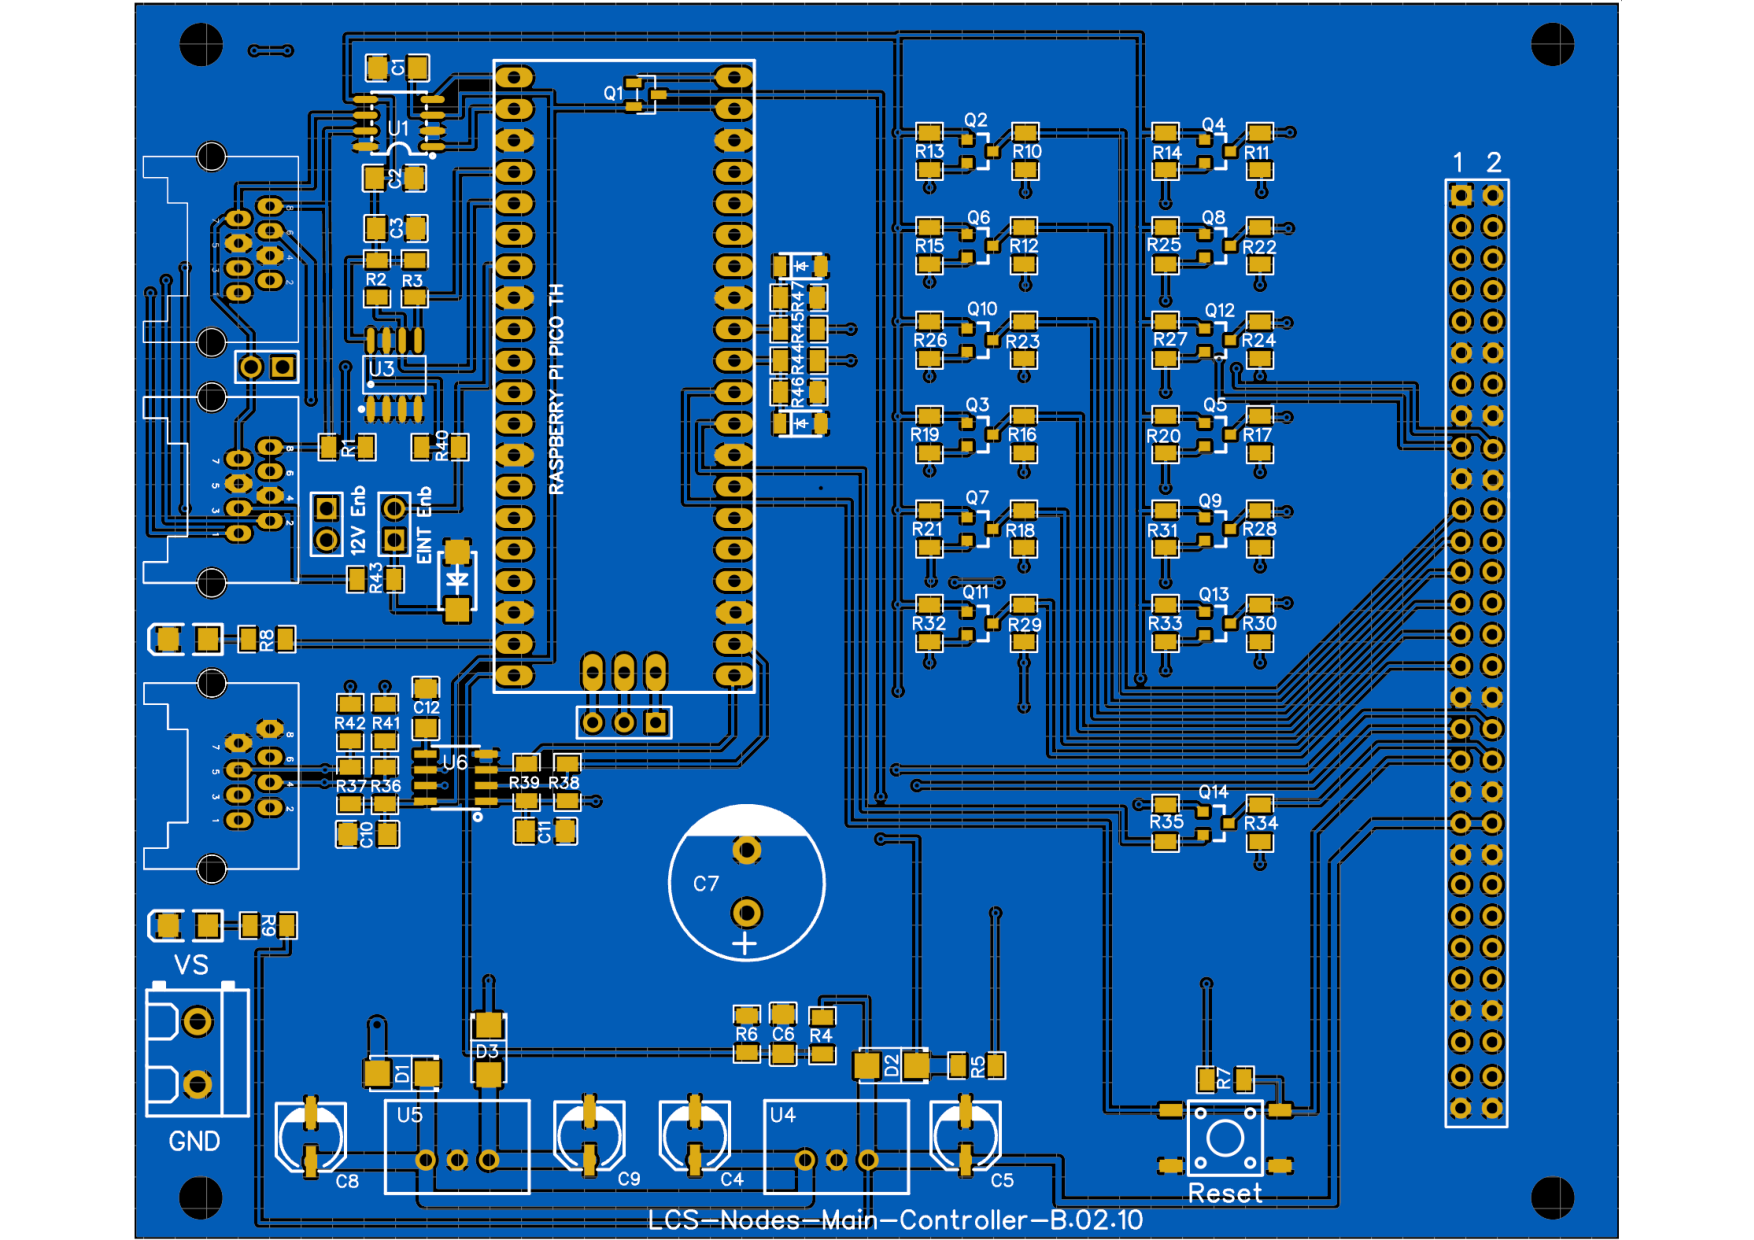
\includegraphics[width=0.8\textwidth]{./part-hardware/chapter-main-controller-hardware-pico/PCB_LcsNodes-Main-Controller-Board-B.02.10.pdf}
    \caption{Main LCS Controller Connector and Level Shifters}
    %\label{fig:schematic}
\end{figure}
\FloatBarrier

A significant portion of the PCB area is used by the 5V to 3.3V level
shifting circuitry. For a fully integrated module where the controller and
the application hardware are located on the same PCB, these level shifters
may not always be required.

For the modular LCS approach, however, they provide a consistent electrical
interface between the controller board and extension boards. This allows
different extension boards to be developed independently while still being
compatible with the same controller platform.

The main controller board therefore represents the basic building block for
many future LCS modules. The following chapters will use this foundation and
add the hardware required for specific tasks such as locomotive control,
track power management and user interfaces.
